\documentclass{article}

\usepackage{amsmath}
\usepackage{mathtools}
\usepackage[utf8]{inputenc}
\usepackage[british]{babel}
\usepackage{csquotes}
\usepackage[T1]{fontenc}
\usepackage{charter}
\usepackage[bitstream-charter]{mathdesign}
\usepackage{natbib}
\usepackage[final,babel]{microtype}
\usepackage[hidelinks]{hyperref}
\usepackage{siunitx}
\usepackage[margin=3pt]{subcaption}
\usepackage{xcolor}
\PassOptionsToPackage{final}{graphicx}

\newcommand{\TODO}[1]{\textcolor{purple}{TODO: \emph{#1}}}

\title{Numerical representation of mountains in atmospheric models}
\author{James Shaw}

\makeatletter
\AtBeginDocument{
  \hypersetup{
    pdftitle = {\@title},
    pdfauthor = {\@author}
  }
}
\makeatother

\begin{document}

\maketitle

I am reaching the end of the first year of my PhD, supervised by Hilary Weller, John Methven and Terry Davies.  The project, `Numerical representation of mountains in atmospheric models', is a continuation of my MSc dissertation, also supervised by Hilary Weller.  My project is CASE sponsored by the Met Office.

The PhD aims to find ways of improving the accuracy of dynamical cores in the presence of orography.  So far, my research has focused on comparing terrain following (TF) and cut cell grids using a series of standard two-dimensional tests.  The results demonstrate the trade-off between the numerical accuracy of pressure gradient and advection terms.  We have submitted an article on this subject to Monthly Weather Review.

This report documents the key results from our comparison of terrain following and cut cell grids and identifies some possible future directions for the project.  During our meeting on November 6th 2015, I'd love to hear your thoughts on my future work, and discuss how my research can help the Met Office.

\section*{Comparison of terrain following and cut cell grids}
We have performed a series of two-dimensional tests using a single nonhydrostatic model to enable a like-for-like comparison.  The model
\begin{itemize}
\item is designed in OpenFOAM CFD for unstructured grids
\item uses an upwind-biased, explicit advection scheme
\item has $\theta$, the Exner function of pressure, and covariant velocities as prognostic variables
\item has a C grid horizontal staggering
\item uses a Lorenz staggering in the vertical
\end{itemize}
The 2D tests use a limited-area domain and Coriolis forces are disabled.  Tests include
\begin{enumerate}
\item Stably stratified atmosphere at rest \citep{klemp2011}
\item Mountain waves \citep{schaer2002}
\item A newly-formulated test of the advection of a stratified thermal profile in a prescribed, terrain-following velocity field
\end{enumerate}
Tests were performed on basic terrain following and cut cell grids.

\subsection*{Stably stratified atmosphere at rest}

\begin{figure}
	\centering
	\footnotesize
	\input{../resting-diagnostics/w}
	\caption{Maximum spurious vertical velocity, \(w\) (\si{\meter\per\second}), in the resting atmosphere test with results on terrain following, cut cell and regular grids.}
	\label{fig:resting}
\end{figure}

A mountain is submerged in a stably stratified atmosphere that is initially at rest.  Numerical errors in calculating the pressure gradient give rise to spurious circulation.  Over orography, metric terms are non-zero and have been documented as a source of error in calculating horizontal pressure gradients \citep{mahrer1984,steppeler2002}.  Errors can be reduced by flattening TF layers or avoiding the metric terms by interpolating pressure onto $z$-levels.

Figure~\ref{fig:resting} shows the maximum spurious vertical velocities induced by pressure gradient errors.  Errors are largest on the terrain following grid.  Accuracy is improved on the cut cell grid but, compared to an orthogonal grid with no terrain, errors are still much larger than round-off.

\subsection*{Mountain waves}

\begin{figure}
	\centering
	%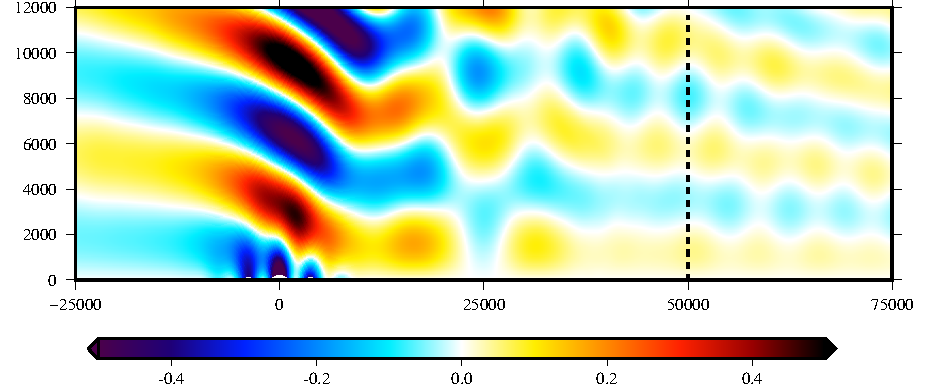
\includegraphics[width=\linewidth]{fig-gravityWaves-theta.pdf}
	\caption{Differences in potential temperature between the start and end of the gravity waves test on the terrain following grid with $\Delta z = \SI{50}{\meter}$.  The dashed line at $x = \SI{50}{\kilo\meter}$ marks the position of the vertical profile in figure~\ref{fig:gw-sampleLine}.  Axes are in units of \si{\meter}.}
	\label{fig:gw-theta}
\end{figure}

\begin{figure}
	\centering
	\footnotesize
	\input{../gravityWaves-diagnostics/sampleLine}
%
	\caption{Vertical profiles of potential temperature differences between the start and end of the gravity waves test on (a) the TF grid, and (b) the cut cell grid.  Results are compared with thermal advection tests results, showing differences in tracer density between the numeric and analytic solutions at the end of integration on (c) the TF grid, and (d) the cut cell grid.  The results are convergent, except for errors found in the lowest layers on the cut cell grids.  \TODO{add GW cut cell dz=50m once the test has completed}}
	\label{fig:gw-sampleLine}
\end{figure}

Following \citet{schaer2002}, gravity waves are induced by flow of over orography.  The test was performed at various resolutions between $\Delta z = \SI{300}{\meter}$ and $\Delta z = \SI{50}{\meter}$ on terrain following and cut cell grids.  The initial potential temperature profile is subtracted from the final field to reveal thermal anomalies.  The result on the terrain following grid at $\Delta z = \SI{50}{\meter}$ is shown in figure~\ref{fig:gw-theta}.  Taking a sample line through the dashed line at $x = \SI{50}{\kilo\meter}$ we compare results between the terrain following and cut cell grids in figures~\ref{fig:gw-sampleLine}a and \ref{fig:gw-sampleLine}b and find that errors are present in the lowest layers on the cut cell grids.  A final advection test is constructed to help establish the source of these errors.

\subsection*{Advection of a stratified thermal profile}

\begin{figure}
	\centering
	\includegraphics[width=3.5in]{tracerDiffMountain.pdf}
%
	\caption{Error in tracer density in the thermal advection test at a resolution of $\Delta z = \SI{50}{\meter}$ on the cut cell grid.  Errors are generated near mountainous terrain and are advected horizontally on the lee side.  Contours in tracer density are overlayed.  Axes are in units of \si{\meter}.}
	\label{fig:thermalAdvection}
\end{figure}

The potential temperature errors in the gravity waves test on the cut cell grids could be caused by
\begin{itemize}
\item differences in velocity fields between TF and cut cell grids
\item error in the advection of potential temperature
\item something else
\end{itemize}
To see if the errors are caused by the advection on cut cell grids, we formulate a new advection test, transporting the initial $\theta$ field from the gravity waves test in a terrain-following velocity field.

A sample line is taken at $x = \SI{50}{\kilo\meter}$ and the results are presented in figure~\ref{fig:gw-sampleLine}c and \ref{fig:gw-sampleLine}d for the terrain following and cut cell grids respectively.  Once again, errors are found in the lowest layers of the cut cell grids, although their magnitude is larger than those in the gravity waves test.  Figure~\ref{fig:thermalAdvection} shows the error field at the end of integration on the cut cell grid at $\Delta z = \SI{50}{\meter}$.  Errors accumulate around mountainous terrain before being advected downstream.

\subsection*{Conclusions}
The key findings are
\begin{itemize}
	\item Pressure gradients are calculated more accurately on cut cell grids
	\item Potential temperature errors are apparent in the lowest layers of the cut cell grid, and these errors are most likely due to advection through cut cells
\end{itemize}
Hence, there is a trade-off between the accuracy in calculating pressure gradient and advection terms.

\section*{Future directions}
Over the last year, our work has prompted us to think of a number of pieces of future work:

\begin{description}
\item[Upwind-biased advection for cut cell grids]{We have made a number of improvements to the upwind-biased cubic advection scheme to ensure that advection remains upwind-biased around cut cells.  The technique is currently implemented in OpenFOAM but is otherwise undocumented.  We could test variants of the advection scheme on cut cell grids to demonstrate the utility of this technique.}

\item[Charney--Phillips staggering for unstructured grids]{Before the advection scheme was improved, zig-zag errors in the gravity waves test lead us to believe that the Lorenz computational mode had been excited.  We started formulating a Charney--Phillips staggering to eliminate these errors, but did not get far enough to obtain results.  We will require further motivation if we want to continue this work.}

\item[TF/cut cell blend]{We have demonstrated that stagnant flows are most accurate on cut cell grids and advection that flows along the terrain is most accurate on terrain following grids.  A grid that blends the two ideas might be able to better represent some types of flow.  For example, we could construct a test that uses cut cells for cold air pools, and terrain-following layers for slope flows.  However, it is not yet clear how such an approach might be generalised for realistic domains.}

\item[`Adcroft for the atmosphere']{\citet{adcroft2013} described a technique for improving the representation of bathymetry.  The approach is designed to model narrow channels without requiring manual intervention, and capture sub-grid scale effects of flow around bathymetry.  \citet{gohm2004} found that very high resolution was required to accurately model gap flows in the atmosphere.  We could apply Adcroft's technique to the land, and we might hope to see improvements to gap flows at coarser resolutions.}
\end{description}
Also, as Terry Davies often reminds us, we must not forget that any dynamical core will need to be connected to parametrizations to be useful, and we must bear this in mind during any future work.

\bibliographystyle{ametsoc2014}
\bibliography{references}

\end{document}
